\documentclass[a4paper,11pt]{article}
\usepackage{a4wide}
\usepackage{graphicx}
\usepackage[utf8]{inputenc}
\usepackage[T1]{fontenc}
\usepackage[czech]{babel}

% vim: spl=cs:


%postup při řešení, způsob řešení
%dosažené cíle
%zdůvodnění případných změn v řešení projektu (technické změny, nikoliv finanční)
%konkrétní výstupy, další využitelnost
%přínosy projektu, vlastní hodnocení
%tisková zpráva – 2 řádky textu (cca 300 znaků) s odkazem na web řešitele

\title{Analýza dat z hmotnostní spektrometrie \\ za použití strojového učení \\[\medskipamount] 
\normalsize
závěrečná zpráva projektu FR CESNET}
\author{Aleš Křenek, Michal Starý, Adam Hájek, (Jiří Novotný)}
\date{\today}

\begin{document}
\maketitle

%\section{Anotace}
\begin{abstract}

Cílem projektu je přenesení prototypů software pro zpracování dat z hmotností
spektrometrie metodami strojového učení na výpočetní zdroje e-INFRA CZ a
vyhodnocení chování těchto algoritmů na dostupných architekturách akcelerátorů
GPU. Práce se zaměří na řešení problémů spojených s velkými objemy dat, jako
třeba distribuované výpočty nebo současné využití více akcelerátorů, a které
bez použití zdrojů e-INFRA nebylo možné řešit. Projekt navazuje na širší
činnost společné výzkumné skupiny centra Recetox a Ústavu výpočetní techniky MU,
která se zabývá mimo jiné i vývojem těchto metod. Přínosem pro aplikační oblast
bude posun ve vývoji prototypů k aplikovatelnosti na rozsáhlé a pro
kompetitivní výzkum nezbytné datové sady. Přínosem pro e-INFRA CZ bude zejména
zkušenost s přenesením a provozem této třídy aplikací na infrastruktuře a
případná zpětná vazba potřebná k jejímu dalšímu rozvoji, jako například
vhodnost konkrétního HW či změny SW prostředí.

\end{abstract}

\section{Postup a způsob řešení}

\subsection{Hmotnostní spektrometrie a strojové učení}

Hmotnostní spektrometrie je experimentální technika, jejíž hlavním cílem je v~základním 
režimu použití potvrzení či vyvrácení přítomnosti konkrétních sloučenin ve zkoumaném vzorku.
Takto je např.\ používána při bezpečnostních kontrolách, kde se zaměřuje na detekci stop manipulace s~výbušninami.

Pro vědecké aplikace je ale významnější a větší výzvu představuje tzv.\ \emph{necílený} (untargeted) režim.
Cílem je zde zjistit pokud možno kompletní složení vzorku přes danou třídu sloučenin (např.\ molekuly daného rozsahu velikosti/hmotnosti).
Použití této techniky je velmi široké, vzorky mohou pocházet z~životního prostředí (půda, voda, i vzduch),
rostlin, potravin, i od lidí (typicky se zkoumají produkty metabolismu, tj.\ vzorky krve, moči a stolice).

\begin{figure}
\begin{center}
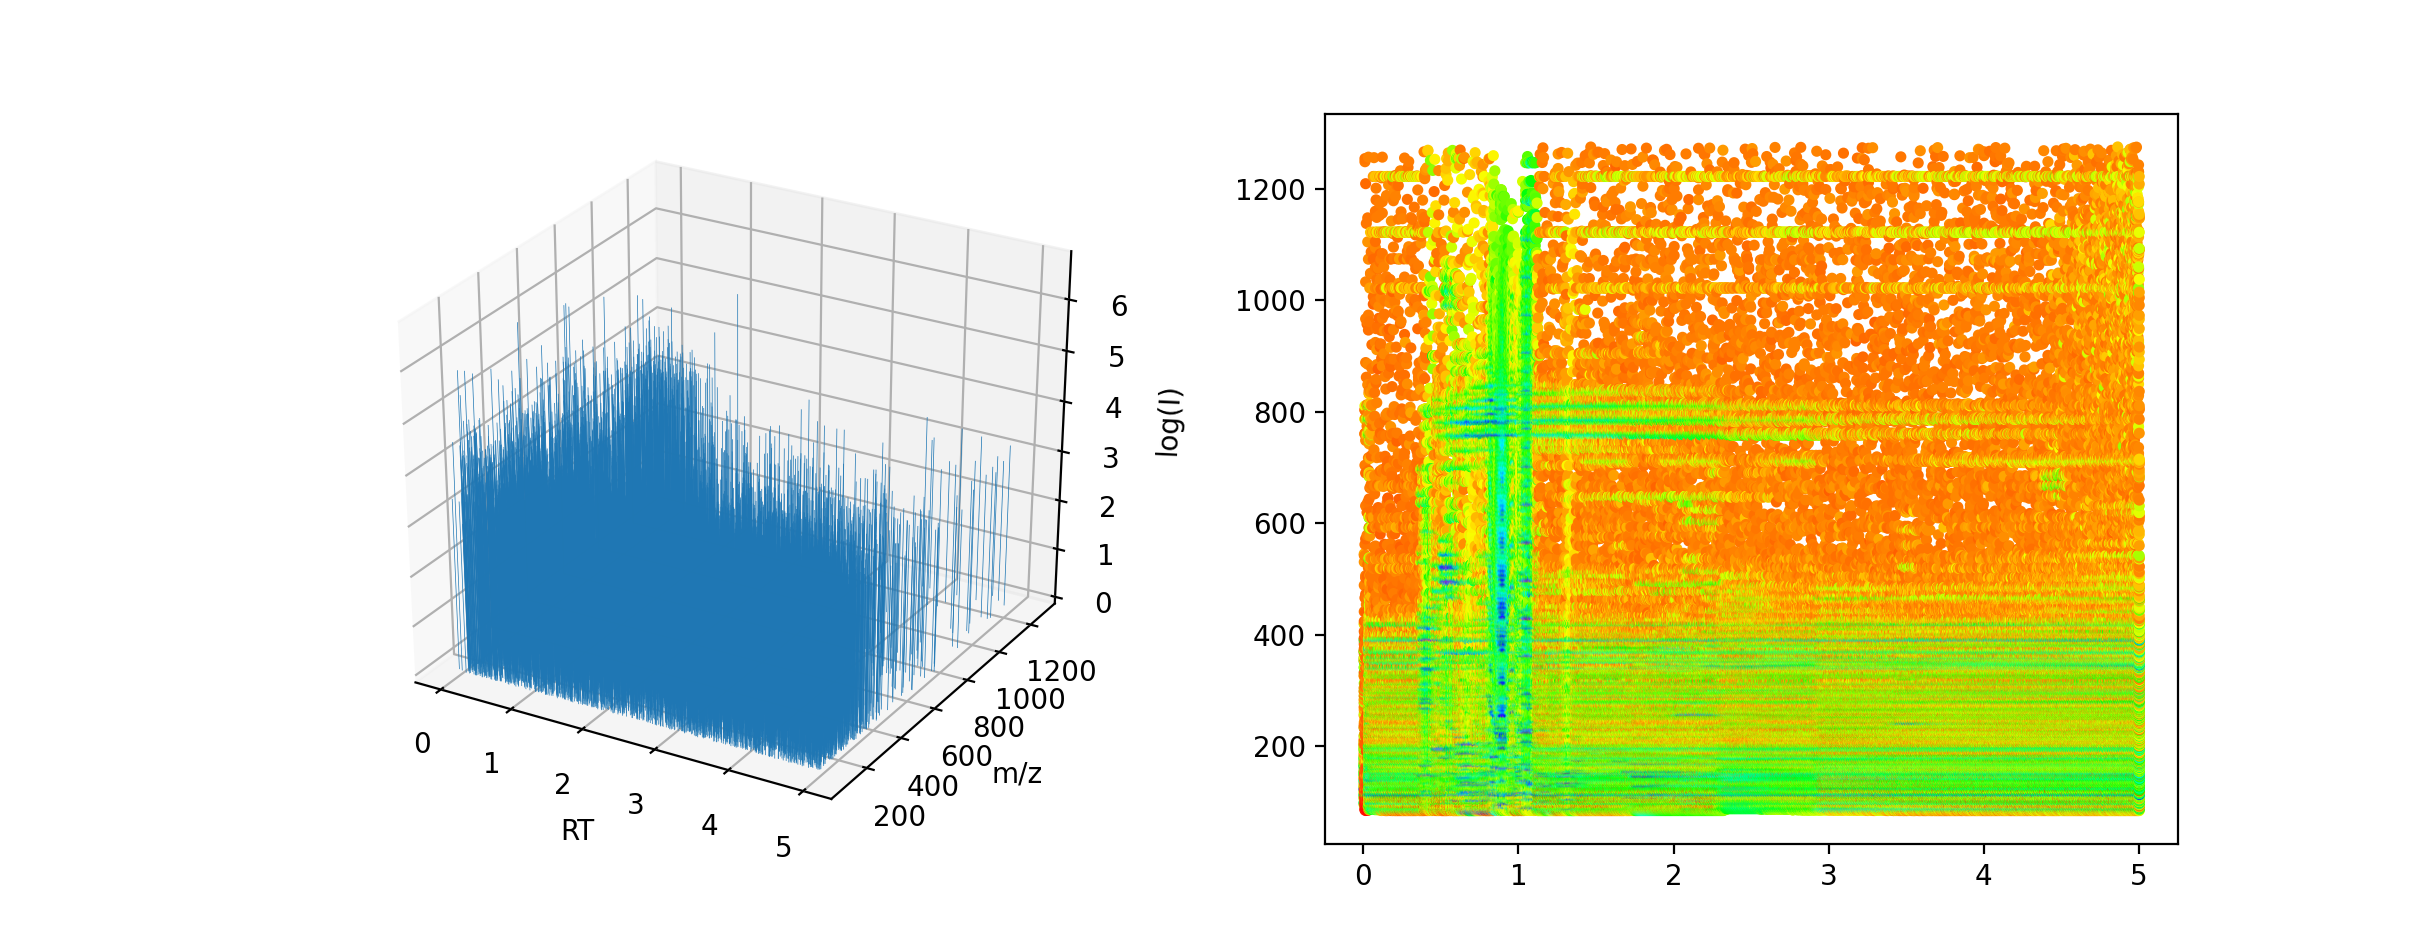
\includegraphics[width=.8\hsize]{sample}
\end{center}
\caption{Ukázka vzorku dat naměřených hmotnostní spektrometrií. Vlevo
třírozměrné zobrazení intenzity signálu pro konkrétní kombinace retenčního času
(\emph{RT}) a hmotnosti ($m/z$), vpravo tatáž data s~barevným kódováním intenzity}
 \label{f:ms}
\end{figure}


Po laboratorním zpracování vzorku (oddělení zajímavé třídy sloučenin, vyčištění, úprava koncentrace \dots)
je typickým dalším krokem kapalinová nebo plynná chromatografie, která od sebe oddělí jednotlivé sloučeniny
ve vzorku, ty se v~konkrétním \emph{retenčním čase} (\emph{RT}) následně dostávají do samotného hmotnostního spektrometru.
Tam jsou nejprve ionizovány, a to buď tzv.\ \emph{měkce},
kdy molekuly pouze získávají náboj a jsou minimálně fragmentovány,
nebo \emph{tvrdě}, kdy je většina molekul ,,rozbita`` na menší elektricky nabité fragmenty.
Pro naše účely (ve spolupráci s~centrem Recetox) se zaměřujeme na druhou variantu.
Hmotnostní spektrometry pak různými způsoby detekují dráhu pohybujících se nabitých částic v~elektrickém poli;
na základě jejich analýzy pak lze určit poměr hmotnosti a náboje ($m/z$) jednotlivých částic.
Jejich souhrn pak tvoří hmotnostní spektrum, které je charakteristické pro konkrétní původní sloučeninu,
a tu tedy lze na jeho základě identifikovat.
Obrázek~\ref{f:ms} ukazuje typická naměřená data.

Data jsou následně výpočetně zpracována (konvenčními metodami), dochází k~odfiltrování šumu, dekonvoluci signálu v~čase,
a korekci artefaktů měření na konkrétním přístroji.
Postupů k~těmto účelům bylo vyvinuto mnoho, a nejsou předmětem tohoto projektu.
Výsledkem pak je posloupnost jednotlivých \emph{hmotnostních spekter}, viz např.\ obr.~\ref{f:thc},
která už patří jednotlivým odděleným sloučeninám.
Konvenční metody pak tato spektra vyhledávají na základě podobnosti v~databázích známých sloučenin,
a~tak jsou sloučeniny identifikovány.

\begin{figure}
\begin{center}
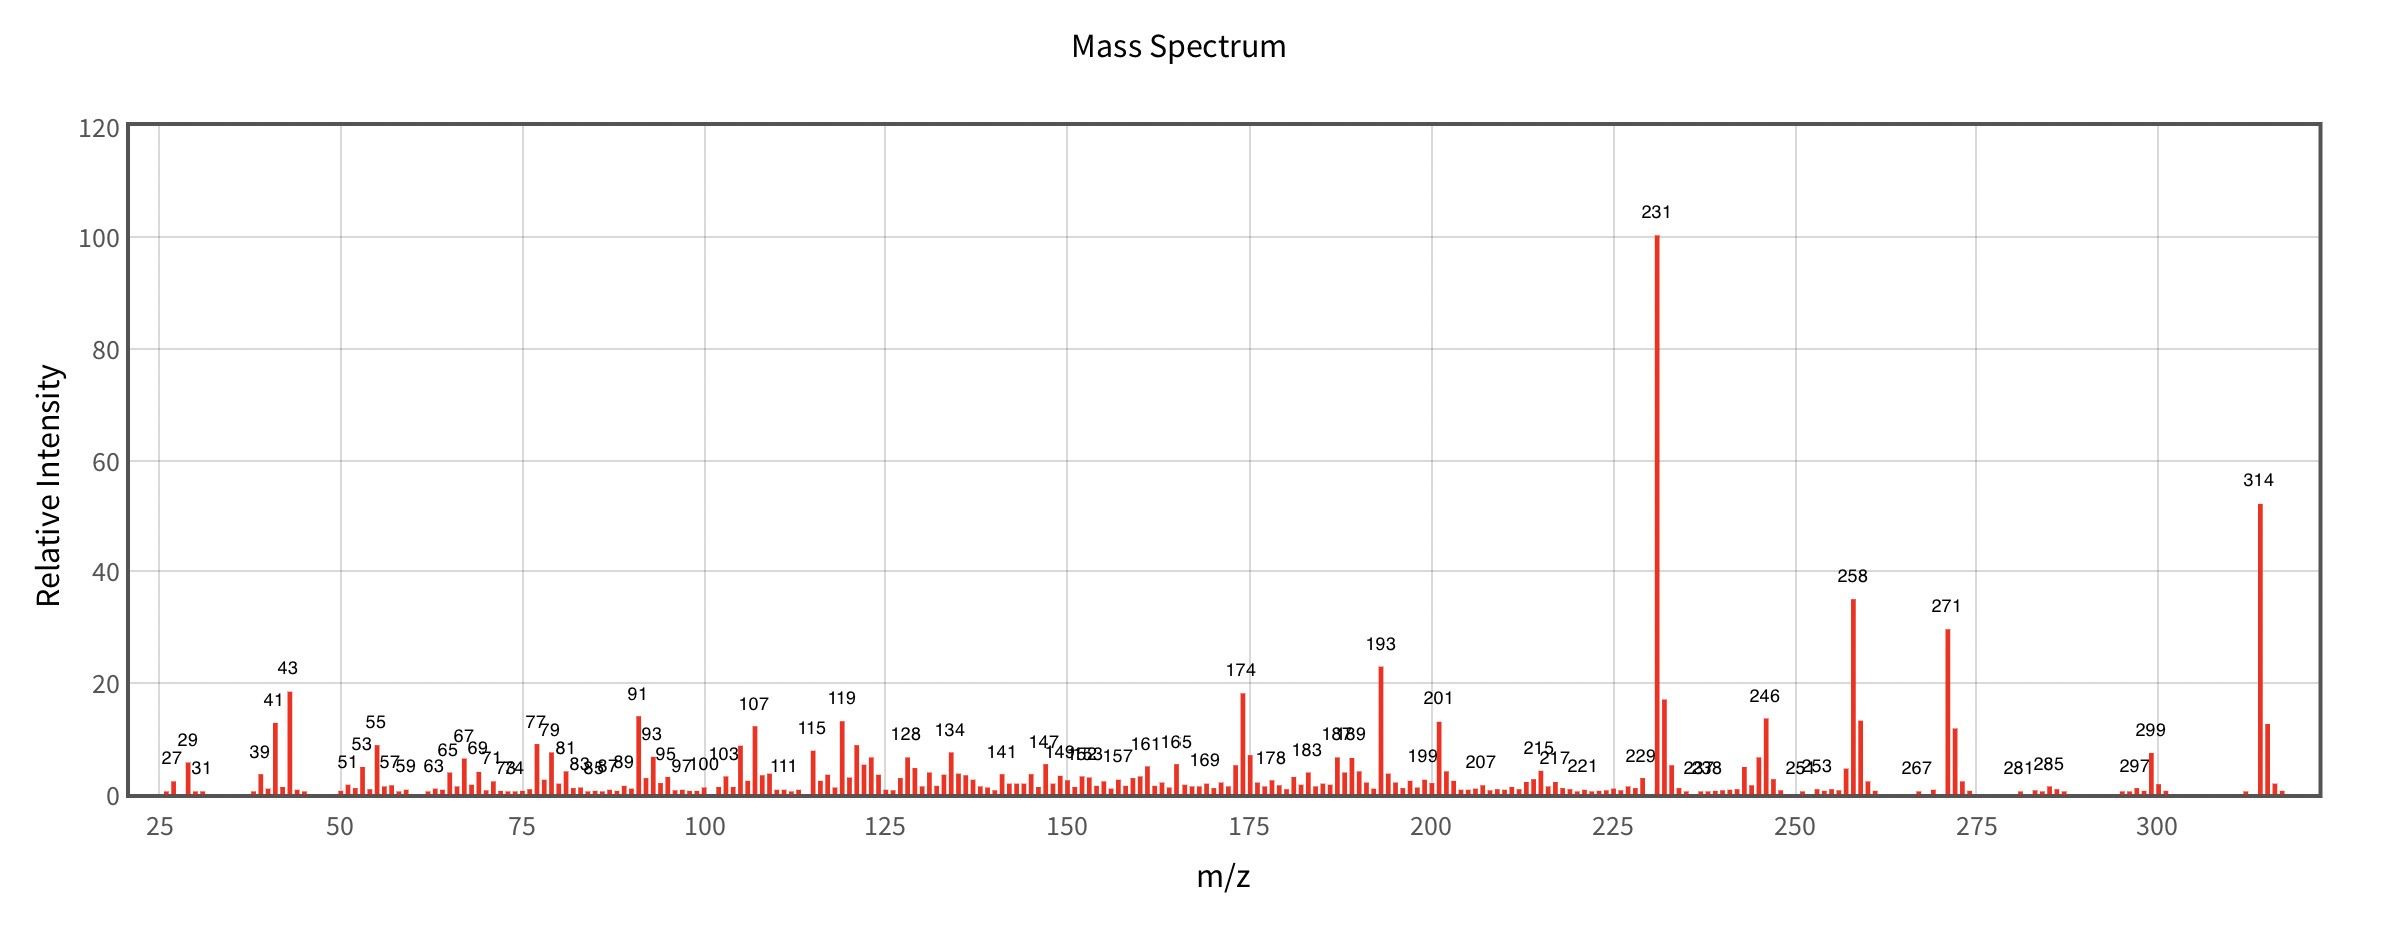
\includegraphics[width=.8\hsize]{thc}
\end{center}
\caption{Ukázka extrahovaného hmotnostního spektra jedné sloučeniny (tetrahydrocannabinol)}
\label{f:thc}
\end{figure}

Výpočetní metody, které realizují výše naznačený postup, jsou komplikované, trpí mnohými nedostatky,
a rozvíjejí se už dekády.
Je tedy zcela přirozené, že v~posledních letech bylo učiněno mnoho pokusů, jak některé nedostatky 
konvenčních metod překonat technikami strojového učení (i jejich stručný výčet by překonal rozsah této zprávy).
V~tomto projektu se zaměřujeme na dvě oblasti, které byly identifikovány ve spolupráci s~centrem Recetox jako potřebné.
Jim jsou věnovány následující části textu.

Pro trénování a vyhodnocení modelů byla použita databáze NIST~\cite{nist}, po předzpracování obsahující
cca.~290~tis.\ záznamů. 
Tato sada byla dále rozdělena na trénovací, validační a testovací,
s~ohledem na skutečnost, že záznamy v~ní nejsou unikátní (v~řadě případů existuje více spekter k~jedné sloučenině) --
zajišťujeme, že sloučeniny reprezentované i různými spektry, se nevyskytují v~trénovací, validační a testovací sadě
současně. 

\subsection{Doplnění chybějícího signálu ve spektrech sloučenin\\ s~nízkou koncentrací}

Zpracování signálu hmotnostní spektrometrie ve fázích odstranění šumu a dekonvoluce je vždy předmětem kompromisu.
Příliš tolerantní nastavení těchto postupů způsobí, že šum, případně přesahy chromatografie v~širším časovém okně jsou
považovány za signál skutečných sloučenin, výsledná spektra jsou příliš ,,zahuštěná`` a následující kroky identifikace
sloučenin jsou pak nepřípustně zatíženy falešnými pozitivy.
Proto je zpravidla nezbytné striktnější nastavení prahů detekce šumu, rozsahu chromatografických špiček a dalších parametrů
zpracování.
V~případě výskytu sloučenin v~nízké koncentraci, což je ale pro mnoho aplikací právě to zajímavé (např.\ běžné metabolity
v~krevní plazmě jsou očekávány i ve vysoké koncentraci, ale hledáme stopy projevů znečištění životního prostředí
pesticidy), metody identifikují slabý signál jako šum, do výsledných spekter se nepromítne, a identifikace je pak zatížena
falešnými negativy.

Řešením tohoto problému se v~projektu zabýval zejména Michal Starý a výsledky jsou i předmětem jeho bakalářské práce.
Identifikovali jsme dva odlišné scénáře -- falešná negativa zanesená příliš agresivní detekcí šumu, kdy jsou ze spekter
chybně odstraněny špičky slabého signálu, a chybějící špičky v~důsledku nedokonalé dekonvoluce, kdy je zpravidla
i relativně silný signál přiřazen do špatného časového okna (tento problém je symetrický, jeho druhou stranou, kdy se 
ve spektru objeví část signálu patřící do jiného času, jsme se prozatím nezabývali, protože pro identifikaci sloučenin
není tak kritický).


% metody
Prvním krokem potřebným pro aplikaci technik strojového učení je vhodná reprezentace 
vstupních dat, tzv.~\emph{embedding}. Použili jsme metodu odvozenou z~publikované metody Spec2Vec~\cite{spec2vec},
která vychází z~technik používaných při zpracování přirozeného jazyka.
Metoda je trénována na reálných datech tak, aby každé špičce přiřadila vektor v~300 rozměrném prostoru tak,
že špičky vyskytující se ve spektrech společně jsou zobrazeny na vzájemně blízké vektory.
Reprezentací celého spektra je pak součet vektorů jednotlivých špiček vážený jejich intenzitou.
Detaily viz příloha~C práce~\ref{stary}.

Pro samotnou predikci chybějících špiček 
uvažujeme danou konstantu $k$ -- počet spolehlivě detekovaných špiček nejvyšší intenzity,
které jsou vstupem predikčního modelu, a jeho úkolem je doplnit (i opakovaně) další. 
Byly vyhodnoceny následující modely:
\begin{itemize}
\item \emph{kNN.} Trénovací sada je zde použita jako databáze, v~níž je vyhledáno $nk$ nejbližších 
záznamů ke vstupu (kde $n$ je hyperparametrem modelu s~použitými hodnotami 1,3,5,10). 
Takto získaná spektra jsou zprůměrována a po vyloučení překryvů se vstupem jsou výstupem špičky setříděné
podle celkové intenzity.
Dalším hyperparametrem metody je metrika použitá k~vyhledávání podobností, používáme cosinovou podobnost
a vzdálenost embeddingu (viz předchozí odstavec).
Tato metoda je jednoduchá a relativně naivní, byla použita zejména pro stanovení startovací čáry pro hodnocení
dalších metod.
\item \emph{LSTM.} Je založena na architektuře tzv.~\emph{Long-Shrt Term Memory}~\cite{lstm} rekurentní neuronové sítě.
Vyzkoušeli jsme tři varianty modelu -- s~náhodnou inicializací embeddingu, jeho předtrénováním, a se zafixovaným embddingem.
Všechny byly aplikovány autoregresivně (výstup jedné iterace je vstupem následující) a přímo, s~extrakcí špiček z~predikované distribuce.
% v Bc 2 hodiny @ A100

\item \emph{GPT-2.} Je postavena na architektuře takto označené architektuře neuronové sítě~\cite{gpt2},
která využívá koncept transformeru.
Nicméně i ,,malá`` varianta používaná pro jazykové modely obsahuje 80 mil.\ trénovaných parametrů,
což je pro naše účely neadekvátně mnoho. Proto používáme redukované varianty s~10, resp. 40 mil.\ parametrů.
Pro špičky (resp. jejich hodnoty $m/z$) je použitý výše popsaný embedding, celé spektrum je zakódováno do vektoru
o 300 složkách.
Podobně jako v~jazykových modelech, kde je dalším vstupním kanálem pořadí slova ve větě,
tímto způsobem do modelu vstupuje intenzita špiček, experimentovali jsme s~jejím kvantováním do 256 úrovní
na lineární a kvadratické škále.
% 10 h @ A100


\end{itemize}

\begin{figure}
\begin{center}
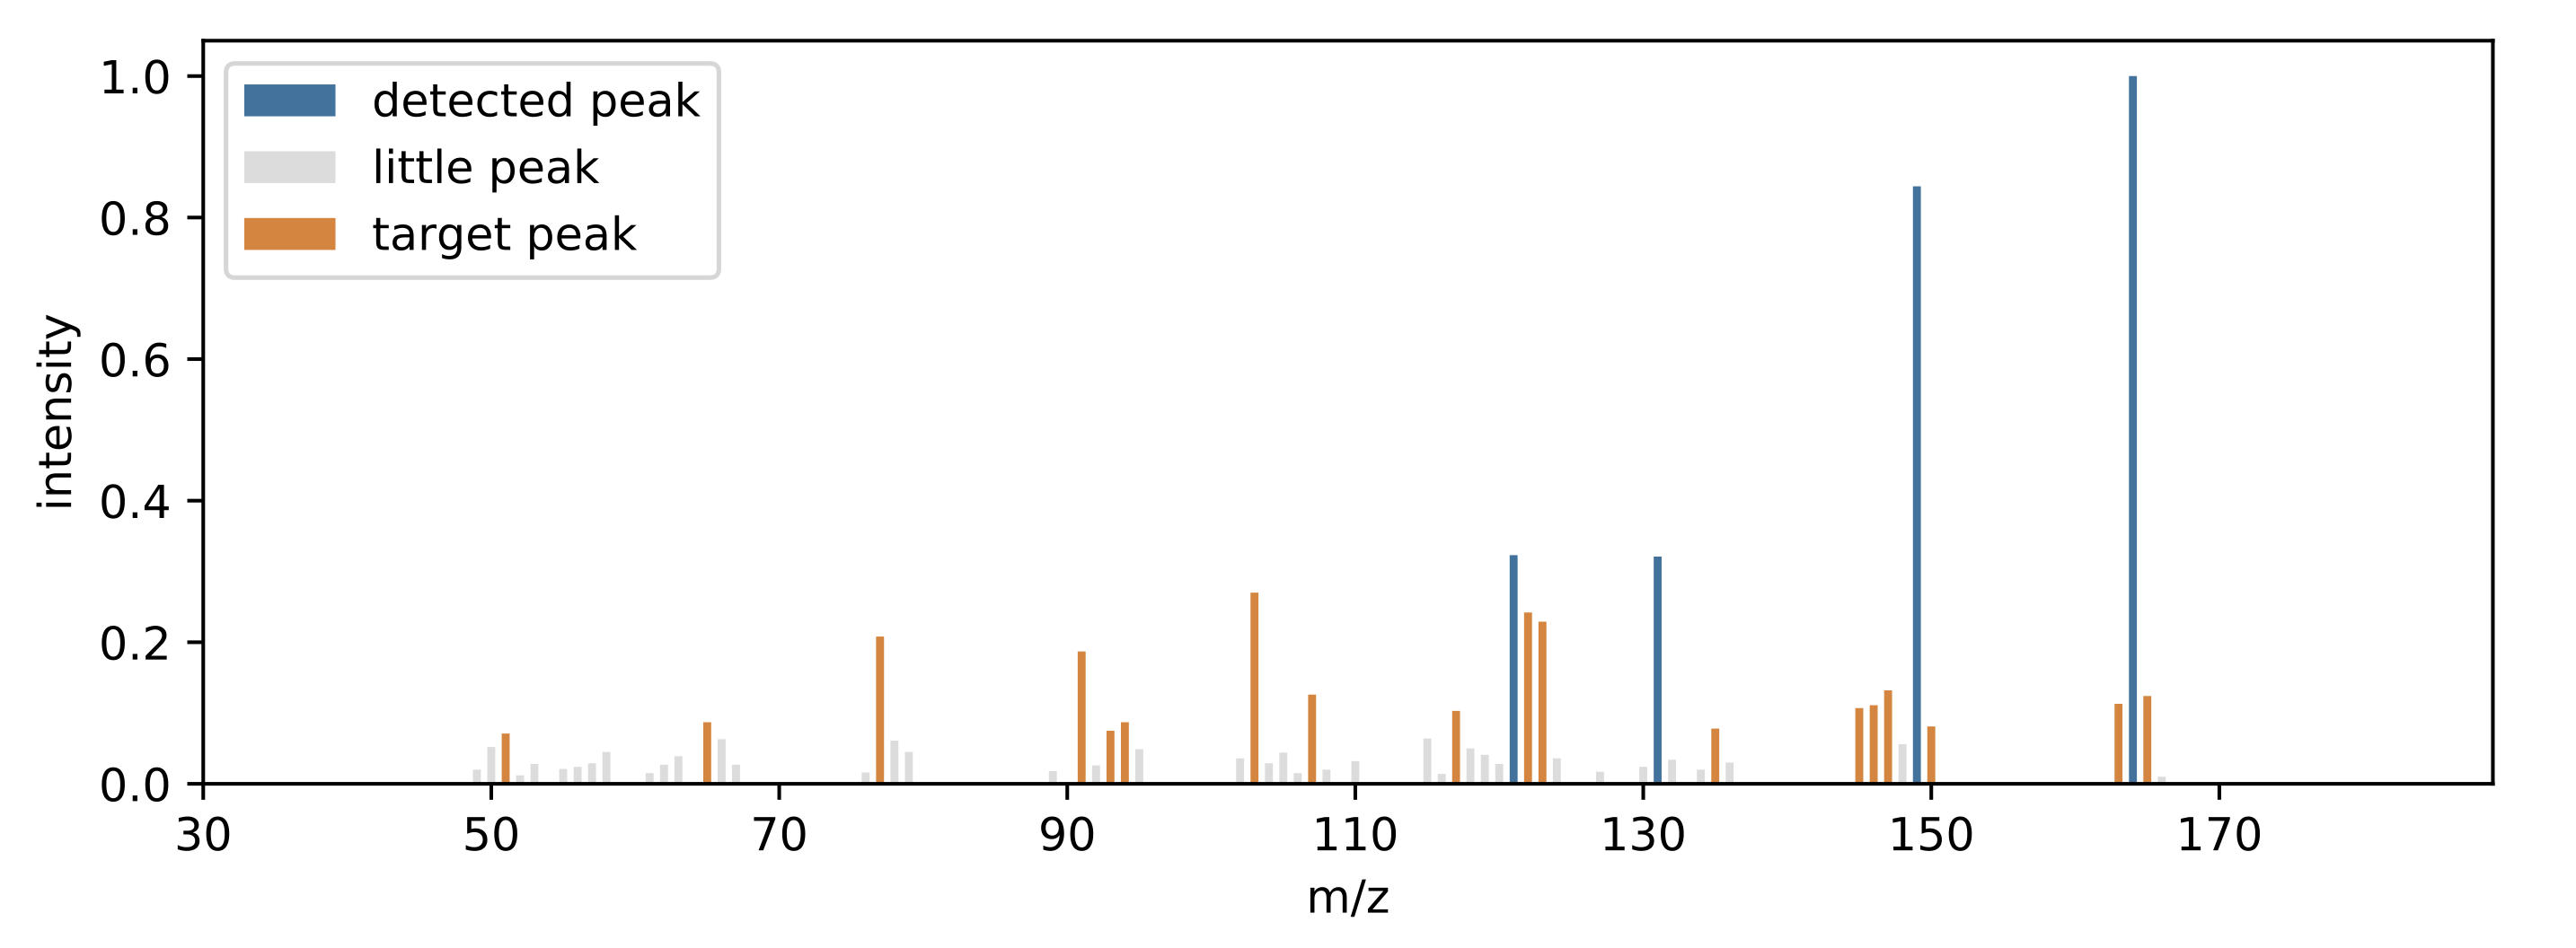
\includegraphics[width=.8\hsize]{metric-missing}
\end{center}
\caption{Konstrukce metriky doplnění chybějících špiček na konkrétním příkladu.
Modře jsou označeny vstupní špičky pro model ($k=4$), oranžově očekávané výsledky.
Pokud např. model detekuje správně špičky na hodnotách $m/z$ 77, 91, 151, 135 (a dalších 14 detekovaných se
s~očekávanými neshoduje), byla přesnost modelu $4/18 = 0.22$
}
\label{f:metric-missing}
\end{figure}

Pro vyhodnocení úspěšnosti a relativní porovnání metod je třeba definovat exaktní metriku.
Neformálně ji ilustruje obrázek~\ref{f:metric-missing}.

Podle dané konstanty~$k$ uvažujeme počet detekovaných špiček, které jsou vstupem pro metodu,
a prahovou hodnotu (empiricky určenou jako 20~\%) relativní intenzity proti $k$-té špičce,
která je ještě považována za významnou. 
U každého testovacího spektra pak identifikujeme množinu špiček, které jsou menší než prvních~$k$,
ale jejichž intenzita je nad prahovou hodnotou, a testovaný model necháme doplnit stejný počet špiček.
Za metriku volíme \emph{přesnost} (precision) této predikce, tj.\ podíl počtu správně identifikovaných špiček
a~celkového počtu očekávaných/doplněných.
Formálně je metrika definována v~příloze~B práce~\cite{stary}. 

Výsledky jsou diskutovány v~části~\ref{cile}.



\subsection{Identifikace neznámých sloučenin.}


% co je MS

% identifikované problémy v MS vhodné pro strojové učení, je jich hromada, nás zajímají tyhle dva

% implementace včetně tech detailů, frameworky, docker, wandb ...

% chybějící peaky ve spektru -- opsané z diplomky

% de-novo identifikace -- co má Adam


% benchmark




\section{Dosažené cíle}
\label{cile}

% vyzkoušelo se několik metod doplnění peaků, fungují docela dobře
% jak to funguje, obrázky z bakalářky

% Michal na tom udělal bakalářku, cena děkana

% transformery pro de-novo identifikaci, prototyp funguje, Adam bude mít diplomku

\section{Zdůvodnění změn}

% JN hodil ručník

% proto prodloužení

% na školení jsme se vykašlali


\section{Konkrétní výstupy a další využitelnost}

% Vlastní softwarový produkt (prototyp)
%• Benchmark + testovací sada
%• Dokumentace k software včetně shrnutí získaných zkušeností a doporučení pro HW/SW
%prostředí
%• Článek shrnující přínos specifického použití metod strojového učení pro aplikační oblast,
%připravený k odeslání do časopisu nebo na odbornou konferenci.
%• Certifikáty ze školení


% implementace chybějících peaků, experimentálně nasazena do Galaxy UMSA

% kód použitelný jako benchmark (github raims)

% prezentace na Metasemináři, Sitole, e-INFRA

% Michalova bakalarka (tam jsou i návody)

\section{Přínosy projektu a hodnocení}

% po útěku JN jsme to stejně zvládli

% navaznost na H2020 EOSC Synergy

\section{Tisková zpráva}

\end{document}
